\documentclass[12pt]{article}
\usepackage[a4paper, margin=2.5cm]{geometry}
\usepackage[dvipsnames]{xcolor}
\usepackage{wrapfig}
\usepackage{graphicx}
%opening
\title{Polymer brush under highly viscous flow}
\author{}
\date{}

\begin{document}

%\maketitle

\begin{center}
	\textcolor{blue}{\huge{Near surface alignment of sheared wormlike micelles}}
\end{center}

\section*{Scientific background}
\begin{wrapfigure}{R}{7cm}
	\centering
	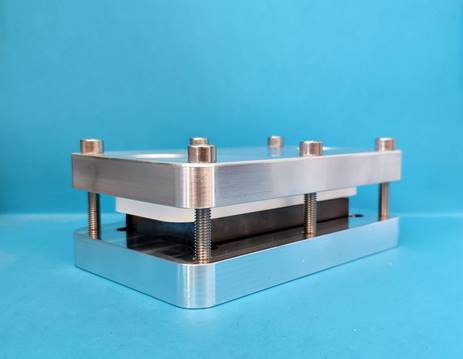
\includegraphics[width=0.4\linewidth]{photo_cell.jpg}
	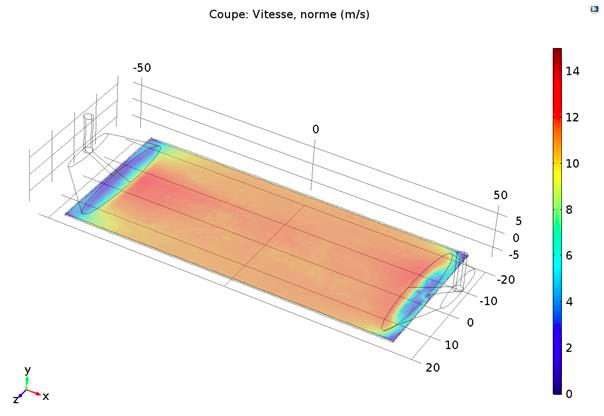
\includegraphics[width=0.4\linewidth]{flow_profile.png}
	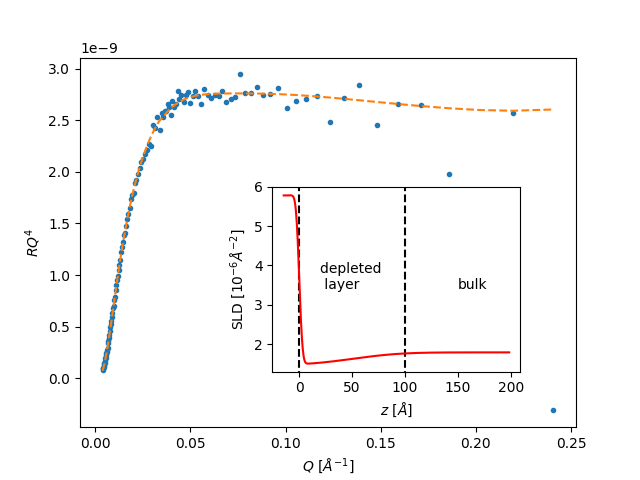
\includegraphics[width=\linewidth]{data_depletion.png}\\
	\textcolor{blue}{\caption{top : Picture of the shear cell shell and flow profile simulated with COMSOL.
			bottom : Neutron reflectivity data and corresponding fit of a sheared polymer solution (PSd/diethyl phtalate 6 wt.\%) in contact with sapphire. The depleted region is insentive to shear rate up to Wi=10.\label{fig:depletion}}}
\end{wrapfigure}


Wormlike micelles (WLMs) are elongated and semi-flexible aggregates resulting from
the self-assembly of surfactant molecules in aqueous solutions which morphology can be controlled by temperature, concentration, salinity and formulation. In semi-dilute regime, WLMs are constantly breaking and recombining leading present a very rich panel of non linear rheological properties highly dependent on their structure (concentration, persistent and contour length...). Several studies have shown that these non linear rheological properties are linked to flow induced structures using Small Angle Scattering, birefringence imaging and ultrasonic velocimetry \cite{berretShearInducedIsotropictoNematicPhase1994, salmonVelocityProfilesShearBanding2003, lerougeShearBandingMicellar1998}. At sufficiently high shear rate, shear bands can appear inducing heterogeneous elongation of WLMs. Thus, rheo-sans and flow birefringence experiments end up with an average signal over the two populations of WLMs.  In the same way, pressure driven flow leads to a heterogeneous shear rate along the fluid gap. Such flow geometry is usually required to study extensional flow \cite{prudhommeElongationalFlowSolutions1994, lutz-buenoMicellarSolutionsContraction2015} and, once again, results in a average signal over WLMs elongation with SANS.
Lettinga \textit{et al.} have investigated the interplay between shear band formation and boundary conditions in worm like micellar systems \cite{lettingaCompetitionShearBanding2009}. They observed no apparent wall slip is observed below the stress plateau because in this region the  flow is stable and gradients at the walls or in bulk do not grow. On the contrary, above the stress plateau, they observed that shear bands do not fully develop over slippery  surface (smooth surface). They suggest that such original features may be due to micellar orientation gradient at the walls but there is to our knowledge no evidence of such an hypothesis.

\section*{Proposed experiment}
Our aim is to probe the near surface structure of wormlike micelle at rest and under shear. In a previous experiment (9-11-2020), we tested a new shear cell we designed using a high viscosity syringe pump allowing to reach Weissenber number up to 20 while ensuring that the shear rate is homogeneous by optimizing the geometry of inlet and outlet nozzle. Thanks to this experimental setup, we evidenced the presence of a polymer depleted layer at the interface which structure is independent from the applied shear rate (Figure \ref{fig:depletion}). In the present proposal, we plan to use cetyltrimethylammonium bromide (CTAB) mixed with Sodium Salicylate (NaSal) co-surfactant. The concentration of CTAB will be fixed at 100mM and the molar ratio between CTAB and NaSal will be varied from 0.2 to 0.4 in order to probe the influence of the contour length and entanglements of the WLMs\cite{lutz-buenoViscoelasticityEnhancementSurfactant2016}. The solvent here is D2O to get the higher contrast. We plan use depth resolved grazing incidence time of flight neutron scattering (ToF-GISANS) on the SANS2D beamline in order to probe the in-plane structure if WLMs \cite{wolffDepthResolvedGrazing2014}. Compared to shear setup based on a rheometer, our flow cell allow probe the GISANS signal parallel and perpendicular to the flow by rotating the flow cell. Thanks to this strategy, the startup of anisotropy as a function of the flow rate can be observed in both directions.


% On the other hand neutrons are totally reflected for a momentum transfer smaller
%than Qc = 0.124 nm−1. This implies that for an incident angle of 0.3◦ the critical wavelength
%for total external reflection is λc = 0.53 nm. Wavelengths longer than λc are totally reflected
%4
%SLD Neutron
%SLD x-ray
%Silicon 2.08*10−6 Å−2 20.1*10−6 Å−2
%Sample 5.17*10−6 Å−2 9.35*10−6 Å−2
%TABLE I. Neutron scattering length densities and electron densities for the interface studied in
%the present work.
%with only the evanescent wave penetrating the sample, whereas shorter wavelength neutrons
%are refracted and transmitted into the liquid.


%\begin{figure}
%	\centering
%	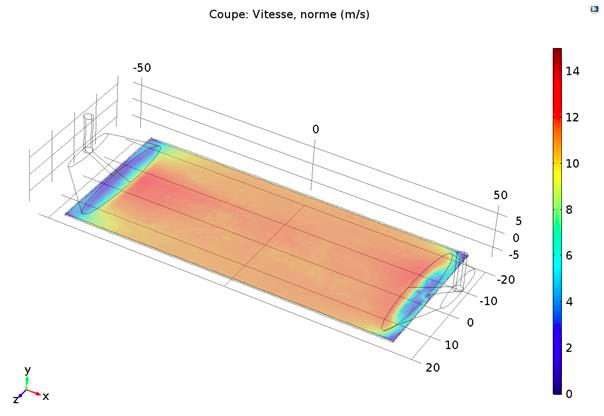
\includegraphics[width=0.7\linewidth]{flow_profile}
%	\caption{}
%	\label{fig:flowprofile}
%\end{figure}
\section*{Beam time justification (3 days)}
In order to probe a large $Q$ range, specular reflectivity measurements will be performed at two angles (0.6° and 2.7°). Two brushes (and 2 spares) with different grafting densities will be studied in contact with 3 polymer solutions (3, 6 and 10 wt. \%) with two contrast conditions (grafted chains matched and free chains matched). For each condition, we plan to exert 5 different flow rates (Wi=0, Wi=0.1, Wi=1, Wi=20 and Wi=0). This results in 60 measurements and 12 changes of sample. The use of two polymer brushes will allow us to optimize the beam time by measuring the one sample will the other is rinsed and dried. Addtionnaly, dry brush measurement before and after the shear experiment will be performed to check that no chains have been detached from the substrate. Taking into account the time for sample alignment, installation of the shear cell setup, we ask therefore for 3 days of beam time on D22.

\bibliographystyle{abbrv}
\scriptsize \bibliography{biblio.bib}
\end{document}
